\chapter[Implementazione]{Implementazione}
Il software si pone l'obiettivo di verificare se una query sia abitata o meno. Esso è formato da due componenti: un modulo Reasoner, scritto in Java che utlizza il reasoner HermiT\cite{HermiT} per stabilire l'abitabilità delle query, e un modulo scritto in OCaml che si occupa di parsare la query da un file testuale, genereare gli assiomi di Leinberger\ref{fig:LeinbergerAxiom} e richiamare il modulo Reasoner. 
    
    \section{-Reasoner}
        Il modulo -Reasoner utilizza due risorse: 
            \begin{enumerate}
                \item Il file HermiT.jar \cite{HermiT}, che implementa il reasoner sviluppato dall'università di Oxford, capace di eseguire ragionamenti sulle ontologie.
                \item Il file DLQueryExample \cite{DLQueryExample} utilizzato per parsare una stringa in una ClassExpression, che è utilizzabile HermiT. 
            \end{enumerate}

        Ma come funziona il modulo? Esso prende in input, in formato stringa, una lista di assiomi di Leinberger, ognuno forma \(A_{x} : C\), con semantica \( A_{x}\sqsubseteq C \). 
        \\\(A_{x}\) è un concetto atomico. "C" è scritto nella "Manchester OWL syntax"\cite{ManchesterOWLSyntax}, e viene trasformato dal DLQueryParser in una ClassExpression. 

        Utilizzando poi la OWLDataFactory (factory delle OWLApi che permette la costruzione di OWLAxiom e di dichiarare OWLClass) e HermiT\cite{HermiT}, dichiariamo all'interno dell'ontologia tutti i concetti atomici, corrispondenti alle variabili della query, che compaiono negli assiomi di Leinberger. 

        \begin{figure}
            \centering
            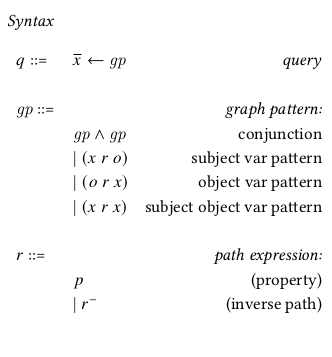
\includegraphics[width=\textwidth]{pictures/leinbergSyntax.png}
            \caption{Codice di dichiarazione degli atomic concept con HermiT}
            \label{fig:declarationCode}
        \end{figure}
                
        Successivamente per ogni assioma creiamo un OWLSubClassOfAxiom, in cui viene specificata ogni concetto atomico come SubClass della sua ClassExpression corrispondente. 

        Infine chiediamo al reasoner HermiT di testare la soddisfacibilità di ogni concetto atomico presente negli assiomi di Leinberger. Se sono tutte soddisfacibili, allora significa che la query è abitabile, altrimenti non lo è.

        \section{-OCaml Module}
        L'idea alla base del modulo OCaml è la seguente: 
            \begin{enumerate}
                \item l'utente inserisce la query di cui testare l'abitabilità in un file di testo. 
                \item la query viene parsata in un tipo Query
                \item sul tipo Query vengono inferiti gli assiomi di Leinberger
                \item viene invocato il -Reasoner e gli vengono passati gli assiomi appena inferiti.
                \item il risultato viene mostrato all'utente
            \end{enumerate}

        Per generare il parser, ho utilizzato il programma OCamlyacc, un compilatore di compilatori, ispirandomi alla grammatica delle query descritta da Leinberger. %pagina 19

        Per definire i token che compongono la grammatica invece mi sono avvalso di OCamllex, un generatore di lexer. 

        Dunque, come funziona il Parser? Esso riconosce la grammatica e genera un tipo Query, che racchiude tutte le informazioni presenti allinterno della query in formato testuale. 

        Per esempio, scrivendo questa query sul file di input: 
        
        $$ query \ x \ <- \ (x \ type \ Pizza \ AND \ x \ hasTopping \ y \ AND \ y \ type \ GorgonzolaTopping) $$
        
        otteniamo il seguente tipo Query così costruito: %mettere?

        $$ Q \  (V \ x, \\
            CP(SP(V \ x,\ TYPE, \ ,\ CP)$$

        Successivamente, il tipo Query viene convertito in una lista di Axiom dalla funzione axiomiserQuery, che implementa le regole di derivazione di Leinberger\ref{fig:axiom}

        \begin{figure}
            \centering
            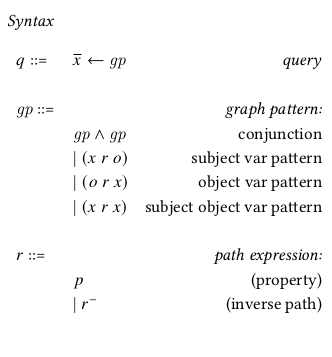
\includegraphics[width=\textwidth]{pictures/leinbergSyntax.png}
            \caption{Sintassi delle query accettata}
            \label{fig:LeinbergerSyntax}
        \end{figure}

        \begin{figure}
            \centering
            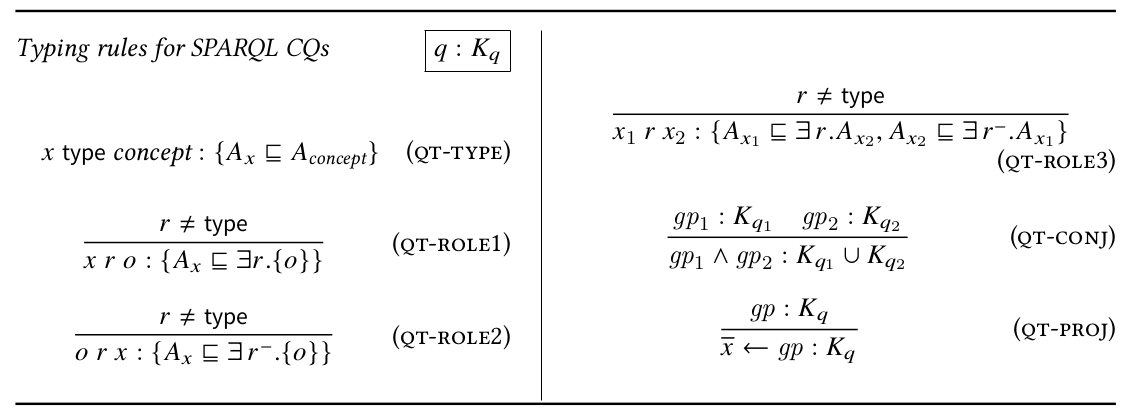
\includegraphics[width=\textwidth]{pictures/leinbergAxiom.png}
            \caption{Regole di derivazione di Leinberger}
            \label{fig:LeinbergerAxiom}
        \end{figure}

        

        
        Infine, la lista viene convertita in stringa secondo la sintassi \(A_{x} : C\). Viene dunque invocato il -Reasoner e gli viene passato come parametro la lista in formato stringa. La risposta, true o false, viene poi mostrata a video all'utente. 
        